\documentclass[tikz,border=3.14mm]{standalone}
\begin{document}
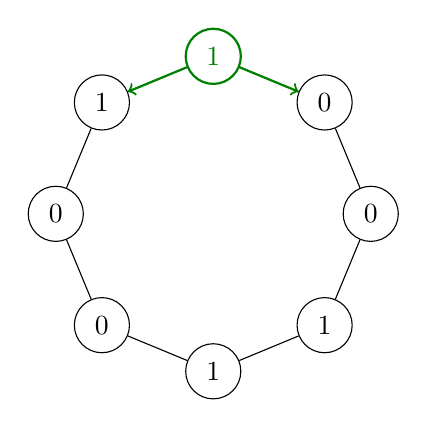
\begin{tikzpicture}[node/.style={draw, circle, minimum size=0.7cm}]
	\definecolor{darkgreen}{rgb}{0.0, 0.5, 0.0}

    % Draw vertices
    \node[node] (v1) at (0:2) {$0$};
    \node[node] (v2) at (45:2) {$0$};
    \node[node, color=darkgreen, thick] (v3) at (90:2) {$1$};
    \node[node] (v4) at (135:2) {$1$};
    \node[node] (v5) at (180:2) {$0$};
    \node[node] (v6) at (225:2) {$0$};
    \node[node] (v7) at (270:2) {$1$};
    \node[node] (v8) at (315:2) {$1$};
    
    \draw (v1) -- (v2);
    \draw (v2) -- (v3);
    \draw (v3) -- (v4);
    \draw (v4) -- (v5);
    \draw (v5) -- (v6);
    \draw (v6) -- (v7);
    \draw (v7) -- (v8);
    \draw (v8) -- (v1);

	\draw[->, darkgreen, thick] (v3) -- (v2);
	\draw[->, darkgreen, thick] (v3) -- (v4);
\end{tikzpicture}
\end{document}
